\chapter{The Runge-Kutta Discontinuous Galerkin Method}
\label{rkdgm}
	This thesis deals with the software \gls{bosss} that uses a \gls{rkdg} method for the numerical approximation of compressible flows. The \gls{rkdg} method is split into the \gls{dg} method for space discretisation and the \gls{rk} method as an explicit time discretisation. By using an explicit time-marching algorithm, the parallelisation is made much easier. \\ \indent
	In the following sections we will study the DG and RK methods separately, considering simple examples and using the same notation as in \textcite{mueller2014}.
	\section{DG Space Discretisation}
		First, we will study the \gls{dg} method which can be seen as combination of the \gls{fvm} and the \gls{fem}. It aims at combining the advantages of both methods, namely high-order accuracy and hp-adaptivity (\gls{fem}), which describes the local refinement of the mesh (h-adaptivity) and of the polynomial degree (p-adaptivity), as well as conservativity (\gls{fvm}), thus allowing the computation of higher order solutions with adjustable order on each element on a conservative grid. The main concept of the \gls{dg} method is visualised in \cref{femfvm}.
		
		\begin{figure}[htp]
			\centering
			\begin{minipage}[b]{0.3\textwidth}
				\centering
				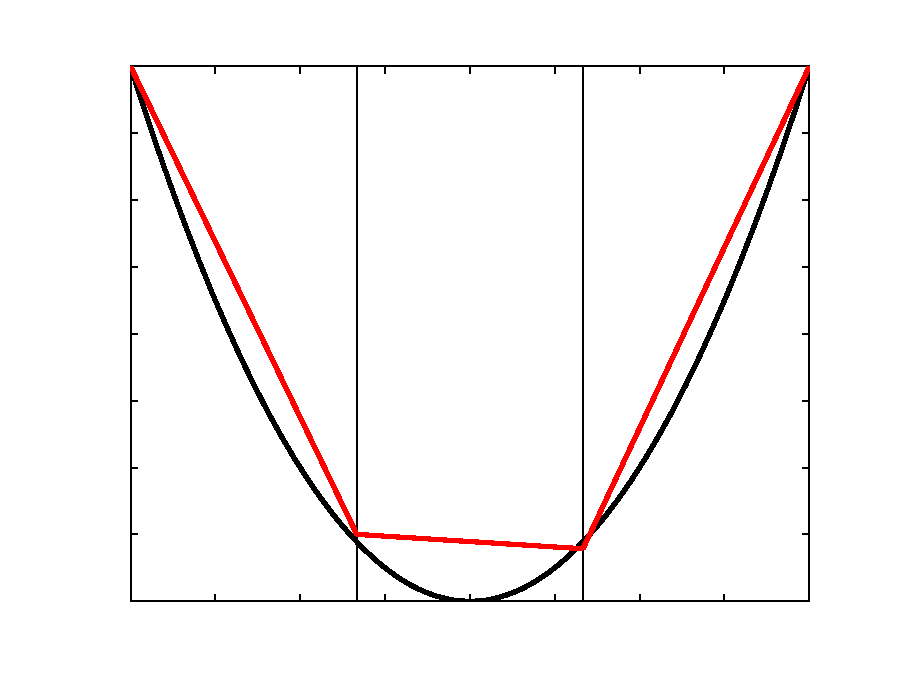
\includegraphics[height=3.3cm]{img/fem.eps}
				\caption*{(a) First order \gls{fem}}
				%	\label{fig:case14gross}
			\end{minipage}
			\quad
			\begin{minipage}[b]{0.3\textwidth}
				\centering
				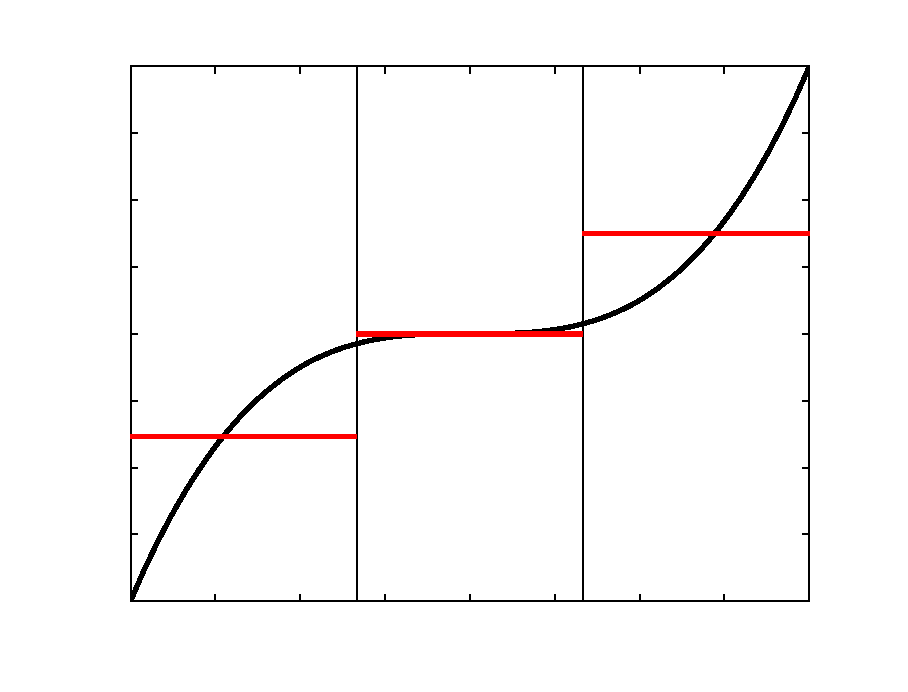
\includegraphics[height=3.3cm]{fvm.eps}
				\caption*{(b) Zeroth order \gls{dg} (\gls{fvm})}
				\label{fig:case1afj4detail}
			\end{minipage}
			\quad
			\begin{minipage}[b]{0.3\textwidth}
				\centering
				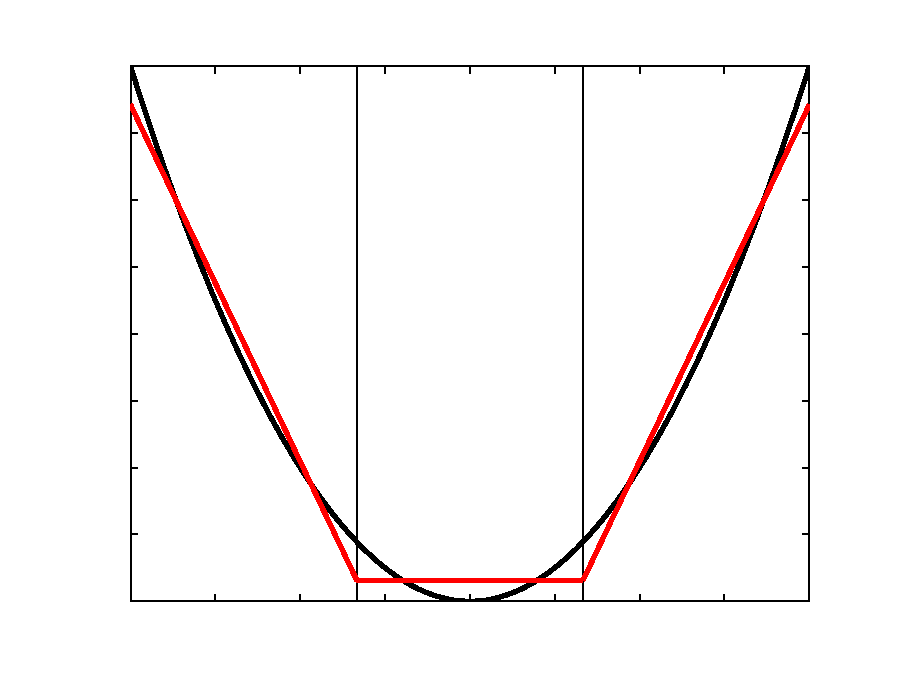
\includegraphics[height=3.3cm]{dg.eps}
				\caption*{(c) First order \gls{dg}}
				\label{femfafdavm}
			\end{minipage}
			\caption{Comparison of \gls{fem}, \gls{fvm} and \gls{dg}}
			\label{femfvm}
		\end{figure}

		As a simple example that we can use in order to derive the \gls{dg} formulation, we will consider the scalar conservation law 	
		\begin{align}
			\frac{\partial c}{\partial t} + \nabla \cdot \boldsymbol{f}(c) = 0
			\label{pde}
		\end{align}	
		for the concentration $c = c(\boldsymbol{x}, t)$  with $\mathbf{x} \in \Omega \subset \mathbb{R}^D$ and $t\in \mathbb{R}_0^+$ and a smooth function $\boldsymbol{f}:\mathbb{R} \rightarrow \mathbb{R}^D$ that also contains suitable initial and boundary conditions.\cite{mueller2014} 
		\subsection{Discrete Weak Formulation}
		Our first step of the DG method will be transferring the partial differential equation \eqref{pde} into a weak formulation.
		Prior to this, we need a discretisation $\Omega_h$ of $\Omega$ consisting of a tesselation of cells $\left\{ \mathcal{K}_i \right\}_{i=1,...,N}$, where $h$ represents a measure for the size of the cells. Each cell $\mathcal{K}_i$ is of dimension $D$ with an outward unit normal vector $\boldsymbol{n}$. \\ \indent 
		After having discretised our geometry, we need a set of cell-local test functions $\left\{\Phi_{i,j}\right\}_{j=1,...,M} $ with $\Phi_{i,j}=\Phi_{i,j}(\boldsymbol{x}):\mathbb{R}^D\rightarrow\mathbb{R}$ that forms the basis of the polynomials $P_{\mathcal{K}_i}(P)$ with maximum degree $P$. \\ \indent
		In order to obtain the discrete weak formulation, we will now multiply equation \eqref{pde} by $\Phi_{i,j}$, integrate over a cell $\mathcal{K}_i$ and then integrate by parts:	
		\begin{gather}	
			\begin{aligned}
			\dfrac{\partial c}{\partial t} + \nabla \cdot \boldsymbol{f}(c) &= 0 \\ 
			\dfrac{\partial c}{\partial t}\Phi_{i,j} + \left(\nabla \cdot \boldsymbol{f}(c)\right)\Phi_{i,j} &= 0 \\ 
			\int\limits_{\mathcal{K}_i} \dfrac{\partial c}{\partial t}\Phi_{i,j} \, dV + \int\limits_{\mathcal{K}_i}\left(\nabla \cdot \boldsymbol{f}(c)\right)\Phi_{i,j} \, dV &= 0\\ 
			\int\limits_{\mathcal{K}_i} \dfrac{\partial c}{\partial t}\Phi_{i,j} \, dV +
			\int\limits_{\partial \mathcal{K}_i} \left(\boldsymbol{f} \left( c \right) \cdot \boldsymbol{n} \right)\Phi_{i,j} \, dA
			- \int\limits_{\mathcal{K}_i} \boldsymbol{f}\left(c\right)\nabla\Phi_{i,j} \, dV &= 0.
			\label{partialintegration}
			\end{aligned}
		\end{gather}
		Considering that the cell's surface $\partial \mathcal{K}_i$ consists of internal or boundary edges $\left\{\mathcal{E}_{i,e}\right\}_{e = 1,...,E_i}$ with
				\begin{align}
				n(i,e) =  
				\begin{cases}
				n & \text{if} ~ \mathcal{E}_{i,e} = \mathcal{K}_i \cap \mathcal{K}_n \\
				0 &\text{otherwise}
				\end{cases}
				\end{align}
		where $n(i,e)=0$ describes a boundary edge, we can rewrite \eqref{partialintegration} as
		\begin{align}
				\int\limits_{\mathcal{K}_i} \dfrac{\partial c}{\partial t}\Phi_{i,j} \, dV +
				\sum_{e=1}^{E_i}\int\limits_{\mathcal{E}_{i,e}} \left(\boldsymbol{f} \left( c \right) \cdot \boldsymbol{n} \right)\Phi_{i,j} \, dA
				- \int\limits_{\mathcal{K}_i} \boldsymbol{f}\left(c\right)\nabla\Phi_{i,j} \, dV &= 0.
				\label{schwacheForm}
		\end{align}
		\subsection{Numerical Fluxes}
		
		As the concentration $c$ is unknown, we need to introduce a modal approximation
		\begin{align}
			c(\mathbf{x} , t)\mid _{\mathcal{K}_i} \approx \bar{c} (\mathbf{x} , t)\mid _{\mathcal{K}_i} = c_i (\boldmath{x} , t) = \sum_{k = 0}^{M}c_{i,k}(t) \Phi_{i,k}(\mathbf{x})
		\end{align}
		with the Galerkin approach of identical Ansatz and test functions. 
		For we do not enforce continuity on $\mathcal{E}_{i,e}$, and thus 
		\begin{align}
			c_i \mid_{\mathcal{E}_{i,e}}=: c^- \neq c^+ := c_{n(i,e)} \mid_{\mathcal{E}_{i,e}},
		\end{align}
		we cannot simply insert the approximation into equation \eqref{schwacheForm}.
		Therefore, we will introduce a monotone, Lipschitz continuous numerical flux function $f = f(c^-, c^+, \mathbf{n}):\mathbb{R}^{D+2}\rightarrow\mathbb{R}$ satisfying the consistency property
		\begin{align}
			f(c^-, c^+, \mathbf{n}) = - f(c^+, c^-, -\mathbf{n}).
		\end{align}
		
		By including these definitions into \eqref{schwacheForm}, we receive
		\begin{align}
			\int\limits_{\mathcal{K}_i} \dfrac{\partial c_i}{\partial t}\Phi_{i,j} \, dV +
			\underbrace{\sum_{e=1}^{E_i}\int\limits_{\mathcal{E}_{i,e}} f \left( c^-, c^+, \mathbf{n} \right) \Phi_{i,j} \, dA - \int\limits_{\mathcal{K}_i} \boldsymbol{f}\left(c_i\right) \cdot \nabla\Phi_{i,j} \, dV}_{=:(\mathbf{f_i})_j} = 0
			\label{schwacheFormFlux}
		\end{align}
		with the discrete operator $\mathbf{f_i}=\mathbf{f_i}(t, \mathbf{c_i})\in\mathbb{R}$.
		
		Some well-known examples of numerical fluxes contain \cite{Cockburn1998}:
		\begin{itemize}
			\item The Godunov flux 
			\item The Engquist-Osher flux
			\item The Lax-Friedrichs flux
			\item The local Lax-Friedrichs flux
			\item The Roe flux with 'entropy fix',
		\end{itemize}
		whereby we will attend to the local Lax-Friedrichs or Rusanov flux, which is defined as
		\begin{align}
			f(c^-, c^+, \mathbf{n}) = \dfrac{\mathbf{f}(c^-)+\mathbf{f}(c^+)}{2} \cdot \mathbf{n} -\dfrac{C_R}{2}(c^+-c^-)
		\end{align}
		with the coefficient $C_R$ based on a local stability criterion. In this thesis, we will use an estimate based on the maximum local wave speed that was developed by \textcite{tororiemann}
		\begin{align}
			C_R = \max(|\mathbf{u^+}\cdot \mathbf{n}|+a^-,|\mathbf{u^-}\cdot \mathbf{n}|+a^+)
		\end{align}
		with $\mathbf{u^\pm}$ and $a^\pm$ denoting the one-sided normal velocity and the local speed of sound.
		As the Rusanov flux has a high stability, it will be used disregarding that it is prone to numerical diffusion.
	\section{RK Time Discretization}
	After having studied the spatial discretisation, we will now attend to the time discretisation, using the \gls{rk} method.\\\indent

	First of all, we need to reformulate equation \eqref{schwacheFormFlux} in order to achieve a system of coupled \glspl{ode}.
	\begin{align*}
		\int\limits_{\mathcal{K}_i} \dfrac{\partial c_i}{\partial t}\Phi_{i,j} \, dV +
		\underbrace{\sum_{e=1}^{E_i}\int\limits_{\mathcal{E}_{i,e}} f \left( c^-, c^+, \mathbf{n} \right) \Phi_{i,j} \, dA - \int\limits_{\mathcal{K}_i} \boldsymbol{f}\left(c_i\right) \cdot \nabla\Phi_{i,j} \, dV}_{=:(\mathbf{f_i})_j} = 0.
	\end{align*}
	
	The first term of the equation above can be reformulated as 
	\begin{align*}
		\int\limits_{\mathcal{K}_i} \dfrac{\partial c_i}{\partial t}\Phi_{i,j} \, dV &= \int\limits_{\mathcal{K}_i} \dfrac{\partial}{\partial t} \left(\sum\limits_{k=0}^{M}c_{i,k}(t)\Phi_{i,k}(\mathbf{x})\right)\Phi_{i,j} \, dV \\
		&= \sum\limits_{k=0}^{M}\dfrac{\partial c_{i,k}}{\partial t}\underbrace{\int\limits_{\mathcal{K}_i}\Phi_{i,k}\Phi_{i,j}\, dV}_{=: (\mathbf{M_i})_{k,j}} \\
		&= \mathbf{M_i} \dfrac{\partial \mathbf{c_i}}{\partial t}
	\end{align*}
	thus leading to 
	\begin{align}
		\mathbf{M_i} \dfrac{\partial \mathbf{c_i}}{\partial t} + \mathbf{f_i} = 0
	\end{align}
	with $\mathbf{M_i}\in \mathbb{R}^{M,M}$ being a cell-local symmetric mass matrix associated with $\mathcal{K}_i$. As we have assumed an orthonormal basis $\left\{\Phi_{i,j}\right\}_{j=1,...,M}$, thus reducing the mass matrix to the identity matrix $I$, the \gls{ode}s simplify to
	\begin{align}
		\dfrac{\partial \mathbf{c_i}}{\partial t} + \mathbf{M_i^{-1}f_i}&=\mathbf{0}\\
		\dfrac{\partial \mathbf{c_i}}{\partial t} + \mathbf{f_i}&=\mathbf{0}.	
	\end{align}
	
	Using an explicit RK method of order S, we can now advance this system of \glspl{ode} and calculate the new coefficients from
	\begin{align}
		\mathbf{c_i}(t_1) = \mathbf{c_i}(t_0)-\Delta t \sum\limits_{s=1}^{S}\mathbf{(\alpha)_s k_s}, 
	\end{align}
	with a known solution at $t_0$ to a new instant $t_1$ and $\Delta t = t_1 - t_0$, where
	\begin{align}
		\mathbf{k}_s = \mathbf{f}_i \left( t_0 +(\mathbf{\beta})_s \Delta t, \mathbf{c}_i (t_0) + \Delta t \sum\limits_{t = 1}^{S}\boldsymbol{(\Gamma)}_{s,t}\mathbf{k}_t\right).
	\end{align}
	
	The coefficients $\alpha \in \mathbb{R}^S$, $\beta \in \mathbb{R}^S$ and $\Gamma \in \mathbb{R}^S$ are specific for each \gls{rk} method. Those of the most common RK methods are displayed in the Butcher Tableaus (\textcite{butcher}, \textcite{gottlieb}) in \cref{RKtableaus}. They determine the stability and accuracy of the time integration scheme. \\ 
\begin{table}[h]
	\begin{equation*}
		% \label{eq:19}
		\begin{array}{l | c c c c c}
			\rule{0pt}{2,3ex} 0      \quad &             &               &              &         &   \\
			\rule{0pt}{2,3ex} \beta_2    \quad & \quad \Gamma_{21}  &              &              &         &   \\
			\rule{0pt}{2,3ex} \beta_3    \quad & \quad \Gamma_{31}  & \quad \Gamma_{32}  &              &         &   \\
			\rule{0pt}{2,3ex} \vdots \quad & \quad \vdots & \quad \vdots & \quad \ddots &         &   \\
			\rule{0pt}{2,3ex} \beta_s    \quad & \quad \Gamma_{s1}  & \quad \Gamma_{s2}  & \quad \cdots & \quad \Gamma_{s,s-1} & \\[2,0ex] \hline
			\rule{0pt}{3,3ex}              & \quad \alpha_{1}  & \quad \alpha_{2}    & \quad \cdots & \quad \alpha_{s-1}  & \quad \alpha_{s}
		\end{array}
	\end{equation*}
	\caption{Butcher Tableau for the Explicit Runge–Kutta Method.}
	\label{tab:RKexplicit}
\end{table}		

\begin{table}
	\centering
	\def\arraystretch{1.5}
	\begin{minipage}[b]{0.18\textwidth}		
		\begin{tabular}{l|c}	
			0 & \\
			\hline
			& 1
		\end{tabular}
		\caption*{Explicit Euler \\(first order)}
	\end{minipage}
	\centering
	\begin{minipage}[b]{0.24\textwidth}		
		\begin{tabular}{l|c c}	
			0 & &\\
			1 & 1 & \\
			\hline
			& $\tfrac{1}{2}$ & $\tfrac{1}{2}$\\
		\end{tabular}
		\caption*{Trapezoidal rule \\(second order)}
	\end{minipage}
	\centering
	\begin{minipage}[b]{0.26\textwidth}		
		\begin{tabular}{l|c c c}	
			0 & & &\\
			$\tfrac{1}{3}$ &$\tfrac{1}{3}$& &\\
			$\tfrac{2}{3}$ & 0 & $\tfrac{1}{3}$ & \\
			\hline
			& $\tfrac{1}{4}$ & 0 & $\tfrac{3}{4}$\\
		\end{tabular}
		\caption*{Third order TVD \\(third order)}
	\end{minipage}
	\centering
	\begin{minipage}[b]{0.29\textwidth}		
		\begin{tabular}{l|c c c c}	
			0 & & & &\\
			$\tfrac{1}{2}$ &$\tfrac{1}{2}$& & &\\
			$\tfrac{1}{2}$ & 0 & $\tfrac{1}{2}$ & &\\
			1 & 0 & 0 & 1 &\\
			\hline
			& $\tfrac{1}{6}$ & $\tfrac{2}{6}$ & $\tfrac{2}{6}$ & $\tfrac{2}{6}$\\
		\end{tabular}
		\caption*{Classical RK \\(fourth order)}
	\end{minipage}
	\caption{Butcher Tableaus for different orders of RK}
	\label{RKtableaus}
\end{table}		
	
	%\captionsetup[table]{labelformat=default}
	
	A well-known stability criterion according the explicit Euler time discretisation for linear, hyperbolic PDEs, namely the \gls{cfl} criterion, restrains the temporal step-size $\Delta t$:
	
	\begin{align}
		\Delta t \leq c_{\text{CFL}} \dfrac{h}{\underline{u}}
	\end{align}
	
	with $\underline{u} \in \mathbb{R}^+$ denoting the largest propagation velocity and a positive constant $c_{\text{CFL}} \leq 1$ depending on the applied spatial discretisation procedure.
	
	Concerning the Euler equations, the largest propagation velocity is given by $\underline{u} = ||\mathbf{u} || + a$ and by taking the influence of the approximation order $P$ into account, we can use the criterion developed by \textcite{cockburn1991runge}
	\begin{align}
		\Delta t \leq \dfrac{c_{\text{CFL}}}{2P+1} \dfrac{h}{||\mathbf{u} || + a}
	\end{align}
	as a sufficiently accurate estimate for the stability criterion in this thesis. 
